\documentclass[a4paper]{article}
\usepackage[utf8]{inputenc}
\usepackage[T1]{fontenc}

\usepackage[backend=biber,sorting=none]{biblatex}
\addbibresource{references.bib}

\usepackage{amsmath}
\usepackage{graphicx}
\usepackage{hyperref}
\usepackage{placeins}

\title{FYS2085 project work: planetary motion}
\author{Mika Mäki}

\begin{document}
\maketitle
\tableofcontents

\section*{Introduction}
The code works as it should, but I ran out of time with the report.


\section{Methods}
The
\href{https://en.wikipedia.org/wiki/Verlet_integration}{Verlet integration algorithm}
is a numerical method for the integration of the Newtonian equations of motion.



\section{Implementation}
The program consists of two parts.
Fortran is used for the computation, and Python for the plotting.

Instructions for building and running the program are available in the readme files in the repository.


\section{Results}
Please see the attached code for interactive 3D visualizations.

\begin{figure}[ht!]
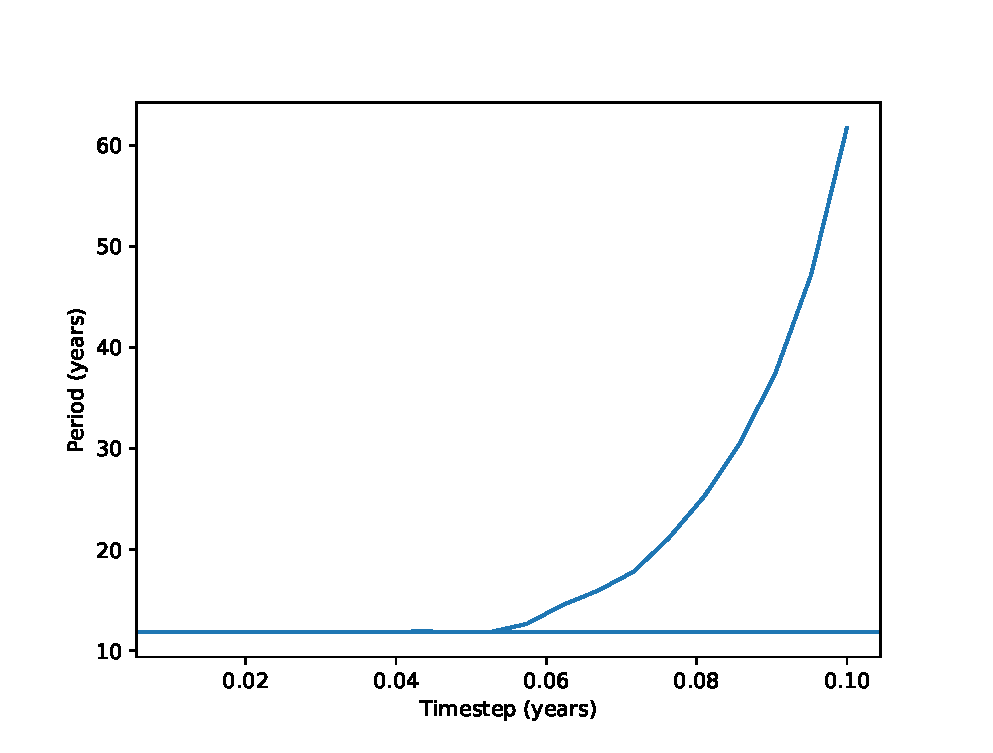
\includegraphics[width=\textwidth]{fig_1a.eps}
\caption{Period of Jupiter's orbit as a function of the simulation timestep (Part 1a)}
\end{figure}

For part 1b the motion of Jupiter was simulated for one orbital period, which was calculated from the radius and velocity of its orbit.
For a simulation timestep of 0.0395 years the rotation during the period was 0.864 degrees too small.


\FloatBarrier
\section{Conclusions}
The simulation works, but there is quite a bit of potential for optimization and further analysis.
It would be fascinating to run the code with a significant number of celestial bodies to model for example a galaxy.

Finally, sorry for the slightly late submission.
I've been doing over 45 credits this semester, so the past few weeks have been very busy.
In case the delay would affect the grade, could I perhaps do
some extra work during the Christmas holiday or submit an improved version of this project
when the course is lectured next year?
(It should be noted that despite the long period available for the project, I was able to start doing it only
a few days ago due to all other coursework and exams,
\href{https://github.com/AgenttiX/planetary-motion/commits/main}{as can be seen in the repository changelog},
and I miscalculated the time it took to get all the bugs ironed out.
)

\end{document}
